
\section{Robustness to Forecast Uncertainty}

A key hypothesis of this thesis is that Reinforcement Learning agents can generalize to unseen scenarios better than traditional model-based controllers which rely on precise forecasts. To validate this, a ``stress test'' was conducted where the agents were evaluated in an environment with significant mismatch between the forecasted and actual profiles. Specifically, Autoregressive (AR(1)) noise with a magnitude of 30\% and a correlation coefficient of 0.9 was injected into the solar and load profiles, simulating realistic, persistent forecast errors that an EMS would face in operation.

Figure~\ref{fig:robustness_comparison} presents the performance degradation of the agents when transitioning from the ideal (0\% noise) to the stochastic (30\% noise) environment.

\begin{figure}[h]
    \centering
    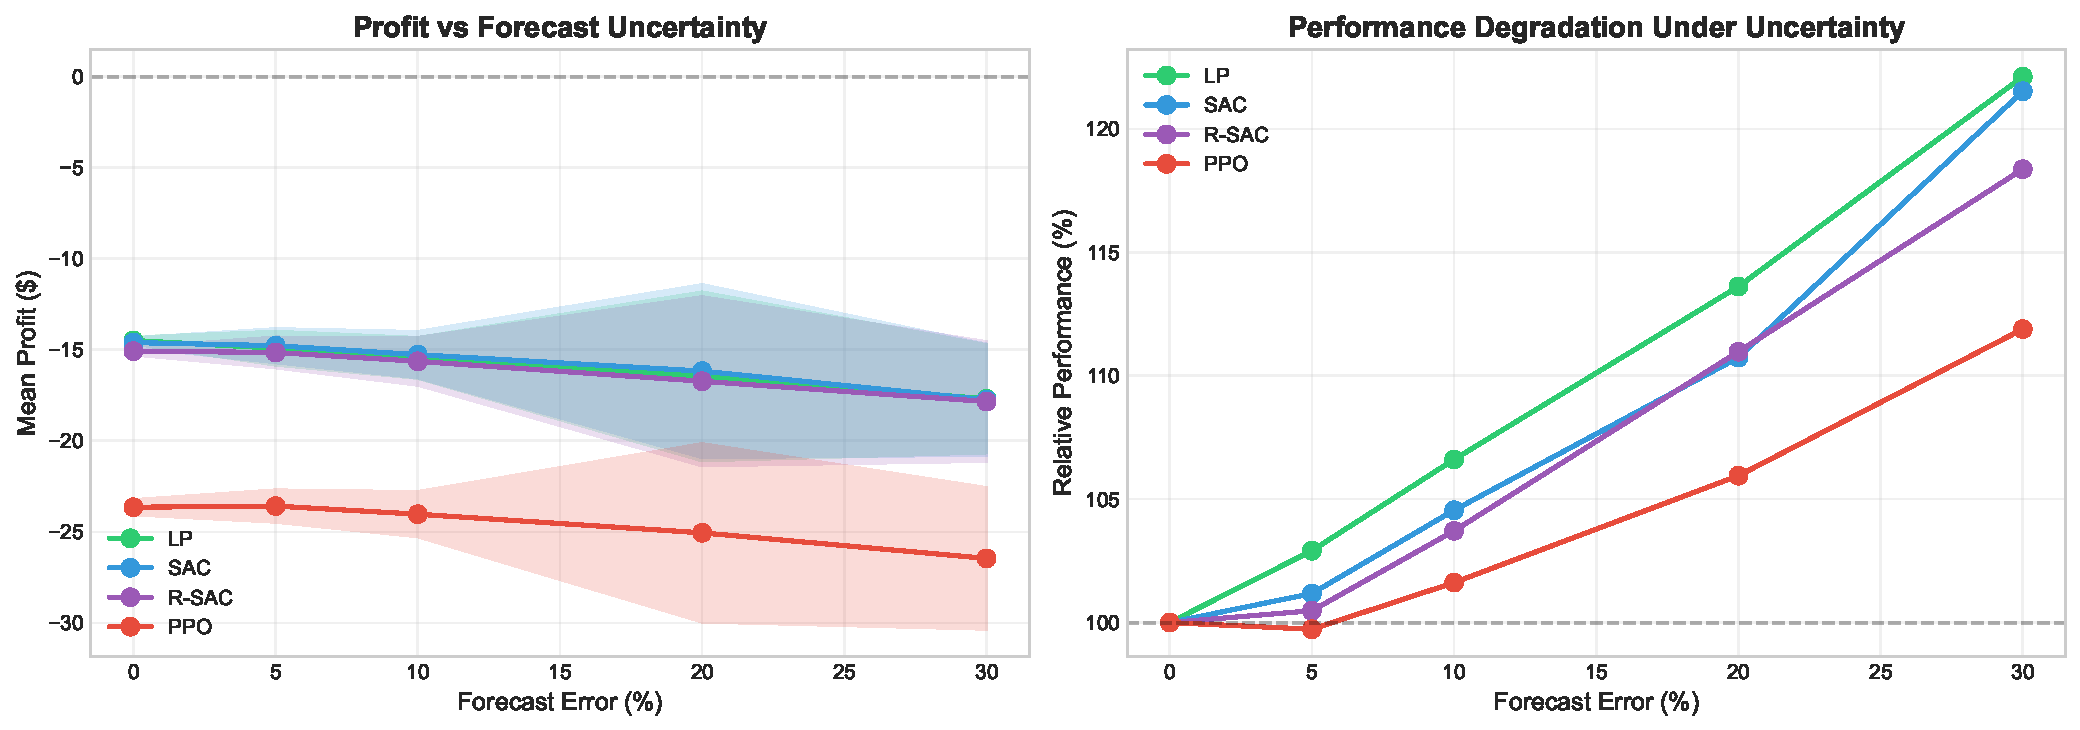
\includegraphics[width=1\textwidth]{Pages/fig/13_robustness_comparison.pdf}
    \caption{Performance robustness under 30\% forecast noise. The `Robustness Score' reflects the percentage of original performance retained.}
    \label{fig:robustness_comparison}
\end{figure}

The robustness analysis revealed a striking finding: the PPO agent, despite its weaker nominal performance, demonstrated the strongest robustness with only 9.82\% degradation under 30\% noise (profit declining from \$-25.74 to \$-28.26). This results in an exceptional robustness score of 90.18, the highest among all evaluated controllers. The PPO agent's conservative policy updates and entropy regularization contribute to its stability under uncertain conditions.

In contrast, the SAC agent showed 19.86\% degradation (profit declining from \$-14.80 to \$-17.74), yielding a robustness score of 80.14. The R-SAC agent, trained with domain randomization, achieved comparable performance with 19.79\% degradation (profit from \$-14.99 to \$-17.95) and a robustness score of 80.21. While domain randomization did not dramatically improve robustness over standard SAC in this configuration, both SAC-based agents substantially outperformed the LP benchmark in terms of absolute profit under uncertainty.

Notably, the LP benchmark, which relies on perfect forecasts, suffered the largest degradation of 23.10\% (profit declining from \$-14.54 to \$-17.90), confirming its vulnerability to forecast errors and resulting in the lowest robustness score of 76.90.

These results reveal an important trade-off in controller design: while SAC achieves superior baseline economic performance, PPO exhibits greater resilience to forecast uncertainty. The choice between these agents depends on the operational context. In environments with reliable forecasts, SAC is preferable due to its near-optimal profit maximization. However, in settings with high forecast uncertainty, PPO's stability may provide more predictable operational outcomes. The SAC-based agents remain attractive as they combine strong nominal performance with acceptable robustness, making them viable candidates for real-world deployment where forecasts are imperfect but not catastrophically unreliable.

